A block diagram of the system model assumed is shown in Fig. \ref{fig:sys_bd}. The system shown in this figure is a downlink system. An access poing (AP) with $N$ transmitting antennas is depicted in the left-hand side of the figure. On the right-hand side of the figure, there are $K$ single-antenna stations (STAs). The MU-MIMO system shown in Fig. \ref{fig:sys_bd} makes use of space division multiple access (SDMA). Each of the $K$ STAs receives its own stream of symbols. The symbols for $STA_i,\ i\in 1,2\ldots,K$ is defined by $s_i$. Before transmission at the AP, each of the $K$ symbols is linearly scaled by a beamforming vector, $\underline w_i$. The $K$ $N \times 1$ vectors are summed together and transmitted over a wireless channel $\underline h_i,\ i= 1,2\ldots K$ to the STAs.
\begin{figure}
    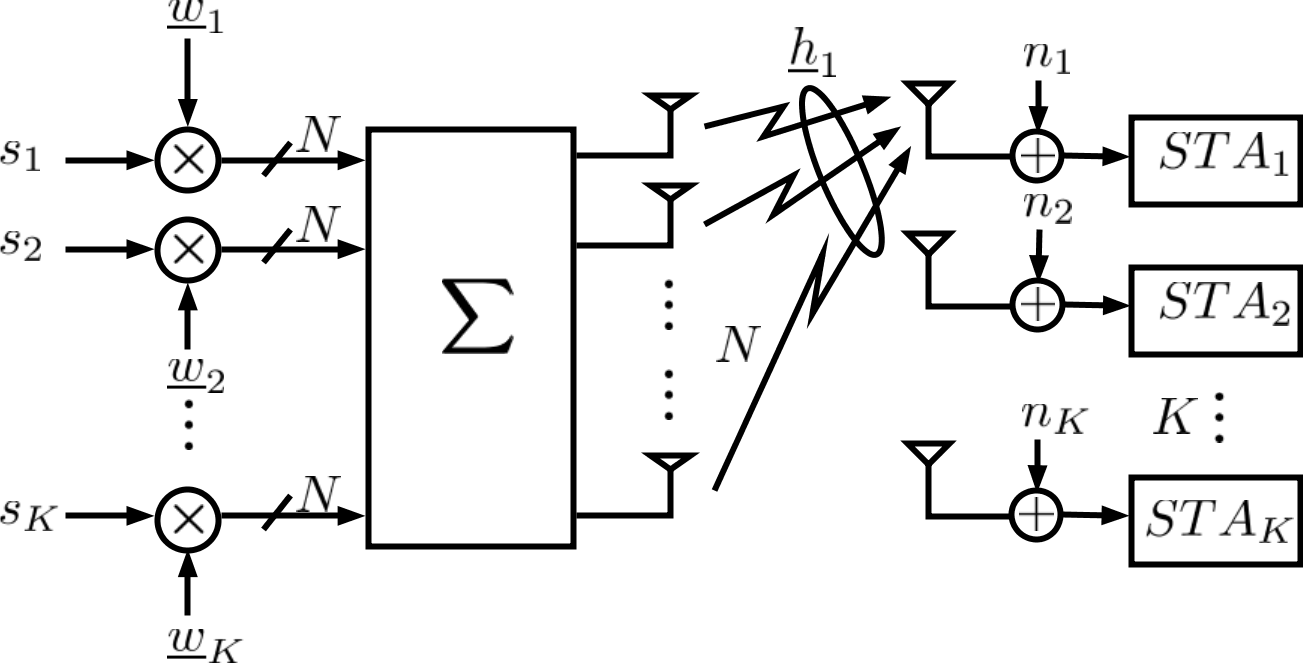
\includegraphics[width=12cm]{figs/system_desc.png}\\
    \caption{Block diagram of the system model.}
    \label{fig:sys_bd}
\end{figure}
